\documentclass[10pt]{standalone}
\usepackage{commands}

\begin{document}
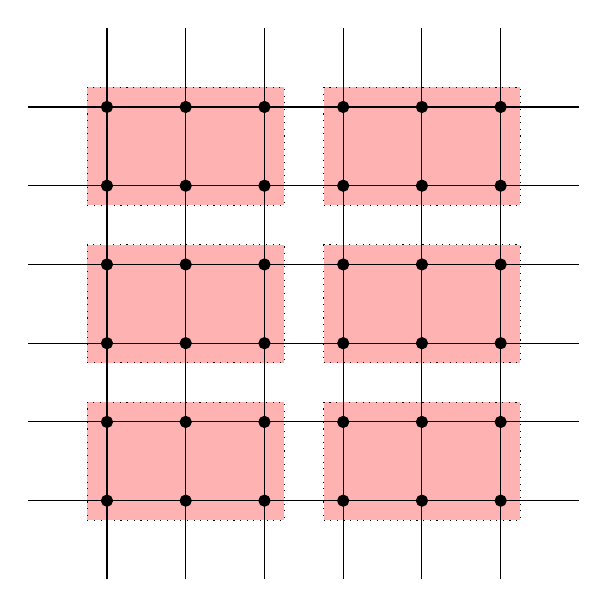
\begin{tikzpicture}
    \foreach \i in {1, 3, 5} {
        \filldraw[dotted, fill=red!30!white!] (-0.25, -0.25+\i) -- (2.25, -0.25+\i) -- (2.25, 1.25+\i) -- (-0.25, 1.25+\i) -- cycle;
        \filldraw[dotted, fill=red!30!white!] (-0.25+3, -0.25+\i) -- (2.25+3, -0.25+\i) -- (2.25+3, 1.25+\i) -- (-0.25+3, 1.25+\i) -- cycle;
    };
    \foreach \j in {1,...,6} {
            \draw[] (-1, \j) -- (6, \j);
    };
    \foreach \i in {0,...,5} {
        \foreach \j in {1,...,6} {
            \filldraw (\i, \j) circle (2pt);
        }
        \draw[] (\i, 0) -- (\i, 7);
    };
\end{tikzpicture}
\end{document}